\documentclass[11pt]{article}
\date{}
\renewcommand\abstractname{\fontsize{14pt}{0}\textbf{Abstract}\selectfont}

\usepackage[left=25mm, right=25mm, top=25mm, bottom=25mm, includehead=false, includefoot=false]{geometry}

\usepackage{graphicx}
\usepackage{url}
\usepackage[round,semicolon]{natbib}  % Citation styles https://www.sharelatex.com/learn/Natbib_citation_styles
\bibliographystyle{apalike}
\renewcommand{\bibsection}{}
\renewcommand{\bibhang}{\setlength{-1px}}


\usepackage{authblk} % For author lists
\renewcommand\Authfont{\fontsize{11}{1}\selectfont}
\renewcommand\Affilfont{\fontsize{9}{1}\selectfont}

\renewcommand*\footnoterule{}

\usepackage[table]{xcolor}
\usepackage[parfill]{parskip} % Line between paragraphs
\usepackage{amsmath}
\pagenumbering{arabic}

\usepackage{sectsty}
\allsectionsfont{\sffamily}

\usepackage[pdftex]{hyperref}
\hypersetup{pdfborder={0 0 0} }


% **************  TITLE AND AUTHOR INFORMATION **************

\title{\sffamily\fontsize{16}{0}\textbf{A spatial simulation model to explore the potential impact of gene drives as a control on invasive wasps}}

\author[1]{David O'Sullivan\thanks{}}
\author[2]{George L. W. Perry}
\author[3]{Phil Lester}
\affil[1]{School of Geography, Environment and Earth Science, Victoria University of Wellington, New Zealand}
\affil[2]{School of Environment, University of Auckland, New Zealand}
\affil[3]{School of Biological Sciences, Victoria University of Wellington, New Zealand}
\affil[*]{\texttt{Email: david.osullivan@vuw.ac.nz}}

\begin{document}

\maketitle

% **************  ABSTRACT  **************

\begin{abstract}
\noindent
\setlength{\parindent}{0pt}
We present a simple simulation model of the potential effects of a possible gene drive control on invasive wasps in the upper South Island of Aotearoa New Zealand.
The aim of the model is to explore the potential spatial dynamics of such a control, in particular, interactions between the distribution of available favourable habitat for wasps, and estimates of their spatial dispersal characteristics.
Preliminary results suggest that even in the absence of an evolutionary response from targetted wasps eradication is unlikely, and that the main determinant of long term abundance of genetically modified strains in the wild population are overall population growth rates.
However, the spatial characteristics of wasp behaviour may have important implications for local eradications and their consequent impact on native wildlife populations.

$ $ \\ {\bf Keywords:} dispersal model, spatial simulation, New Zealand, invasive insects
\end{abstract}


% **************  MAIN BODY OF THE PAPER **************

\section{Introduction}\label{sec:introduction}
It is unclear if gene drives are a viable strategy for control of pest insects.
Laboratory experiments suggest that a gene drive that affects reproduction has the potential to eradicate a species \citep{Galizi2016,Noble2018,Kyrou2018}, while work with simulation models suggests a less optimistic outcome resulting from the evolutionary response of the targetted organism \citep{Bull2016,Noble2018,Unckless2017}.
In this paper we report preliminary results from a spatially explicit simulation model to explore potential effects of a gene drive on invasive wasps.
The results suggest that eradication is unlikely, and that considerably more research is required before gene drive technologies can be considered a viable method of control.
Contrary to expectations, the particular spatial dispersal characteristics of targetted species do not appear to have much effect on long term population outcomes, although the spatial strategies pursued in the release of genetically modified organisms can alter the time taken for new stable population levels to be achieved.
\par
%
%
\section{Model description}\label{sec:model-description}
The model has been implemented in NetLogo, version 6 \citep{Wilensky1999}.
A view of the model interface is shown in Figure~\ref{fig:interface} and serves as a roadmap for the description presented here.
\par
%%
\begin{figure}
  \begin{center}
    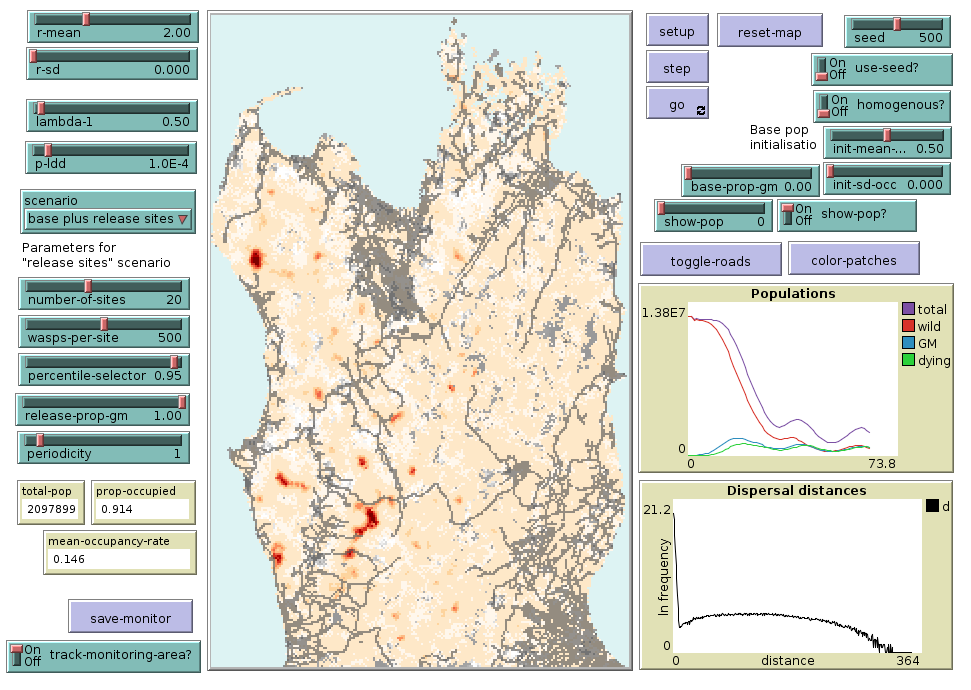
\includegraphics[width=\textwidth]{wasps_interface}
    \caption{The model interface also showing the area of the South Island covered by the model.}\label{fig:interface}
  \end{center}
\end{figure} %
%%
\subsection{Model scope}\label{sec:model-scope}
The model covers the upper South Island of New Zealand.
The region was reprojected to a custom oblique Mercator to reorient the South Island `vertically' reducing the overhead of ocean grid cells in the model where no population is simulated or could arise.
A more conventional projection shows the study area extent in Figure~\ref{fig:locator-map}.
\par
%%
\begin{figure}
  \begin{center}
    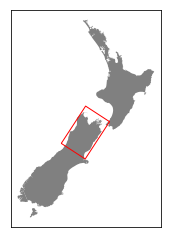
\includegraphics{locator_map}
    \caption{The study area extent.}\label{fig:locator-map}
  \end{center}
\end{figure} %
%%
Within this area a habitat suitability surface at 1 kilometre resolution was derived from the basic ecosystems dataset \citep{BarringerND} such that broad leaved forest cover is assumed to be able to support dense populations, while pasture and grasslands can only much lower populations.
\par
%
Wasp population in each cell falls into three classes, wild, genetically modified, and sterile.
A simple population model represents the spread of a gene drive for sterility through the population, affecting the relative numbers of each of these classes in each new generation, in combination with an overall reproductive rate.
At the end of each season (i.e. each year) queen wasps move according to a dispersal function that favours local dispersal but allows for rare long distance `jumps' (which in the real world might occur as a result of a queen hitching a ride on a logging truck, for example).
\par
%%
\begin{figure}[hbt]
  \begin{center}
    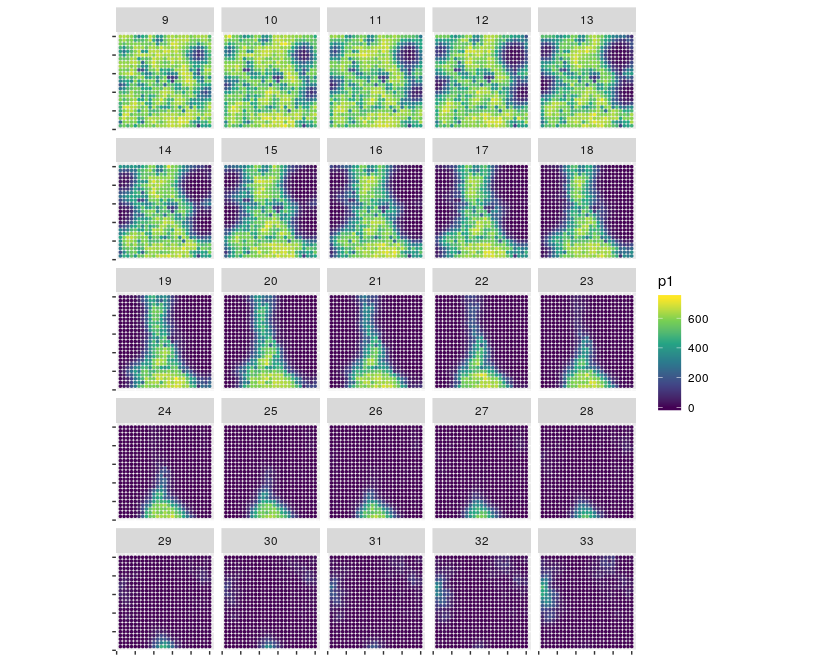
\includegraphics[width=\textwidth]{local_dynamics}
    \caption{Local dynamics of the model in a 25$\times$25km area over a 25 year time frame, showing the slow spread of local extinction.}\label{fig:local-dynamics}
  \end{center}
\end{figure} %
%%
The model allows for a variety of possible control strategies.
Genetically modified wasps with a gene drive can be introduced at a set number of locations determined from the local population of wasps, presumably targetting a number of sites in the upper range of population presence.
Releases can also be made more or less frequent.
The combined effects of demography, dispersal and patterns of release of genetically modified wasps yield shifting patterns of wasp presence across the modelled region.
\par
%
%
\section{Results}\label{sec:results}
Prelminary results from the model will presented at the conference.
\par
Of particular interest are spatial aspects of the model outcomes and whether or not the spatial characteristics of wasp dispersal are likely to have an impact on the potential of this approach to control wasp populations.
A related question is the degree to which, given that eradication on any reasonable time frame is unlikely, local extinctions have the potential to contribute to the recovery of native insect and bird populations.
\par
Preliminary results suggest that wasp population dynamics may ultimately not depend greatly on the spatial characteristics of their dispersal behaviour, rather that demography (i.e., overall reproductive rates) are more significant to long term stable population levels.
The spatial dispersal behaviour of wasps is observable in the spatial dynamics of local extinctions (see Figure~\ref{fig:local-dynamics}), and this may be critical to any potential for ecological benefits for this or similar control technologies, since it affects the time available for native ecosystems to recover from the presence of wasps.
\par
%
%
\section{Acknowledgments}\label{sec:acknowledgments}
This research has been partly funded through the The National Science BioHeritage Challenge, Ngā Koiora Tuku Iko.
%


\section{References}
\bibliography{geocomp2019}


\end{document}
